% mainfile: ../../main.tex
\chapter{Vibration noise}\label{ch:setup:vibrations}
\AutoLettrine{A} microscope's performance is limited chiefly by two factors; first and foremost the resolution and imaging fidelity are limited by the systematic aberrations introduced by the optics.\sidenote{
    Besides the limit set by the wavelength-dependent diffraction, of course.
}
Various types of aberrations exist, and modern microscopes usually include a complex assembly of optics to compensate for these errors.
The second factor is vibration noise.
This becomes more significant the higher the resolution of the microscope simply because ambient, environmental vibrations within the range of human civilization is typically on the order of $\qty{100}{\micro\meter\per\second}$ \gls{rms}~\cite{Gordon1999}.
Comparing that to transmission electron microscopes with atomic resolution, it is clear that these instruments require purpose-built rooms to reduce the vibration level to acceptable levels.

The demands on the microscope discussed in \thethesis are fortunately much more relaxed as the features we need to resolve are on the micrometer scale.
However, we face the additional challenge of ultra-low temperatures, or rather the manner in which they are achieved.
The microscope is integrated into a \emph{dry} \gls{dr}.
In contrast to a \emph{wet} \gls{dr}, which uses a liquid Helium bath, these systems achieve the pre-cooling necessary for the \ch{^3He}/\ch{^4He} dilution refrigeration cycle to work by adding a secondary refrigeration mechanism, a \gls{ptr}.
These are closed-cycle systems that work with \ch{^4He} compressed to \textasciitilde\qty{21}{\bar} on the high-pressure and \textasciitilde\qty{7}{\bar} on the low-pressure side.
A rotating valve connecting high and low pressure lines to the cryostat in turn produces alternating gas flow inside a regenerator, where the gas absorbs heat at the low-temperature and and deposits heat at the high-temperature end~\cite{Radebaugh2009,DeWaele2011}.
In commercial \glspl{ptr} the frequency of the pulses of Helium gas, determined by the rotary valve motor, is usually fixed at values around \qty{1.5}{\hertz}.

Naturally, the compressor, the rotary valve motor, and the Helium pulses themselves introduce vibrations into the cryostat.
While the cold foot of the \gls{ptr} is not rigidly connected to the cryostat interior,\sidenote{
    In the \odin copper braids connect the cold head to the \gls{pt1} and \gls{pt2} plates.
    There exist commercial systems that use gas exchange instead, for example the \mbox{CryoConcept} HEXA-DRY series~\cite{CryoConceptHexaDry}.
}
the entire cold head assembly rests with rubber feet on the cryostat top plate in the system's delivery status.
Thus, our microscope does not only encounter passive environmental vibrations but also the active perturbation from the \gls{ptr}.

Several authors have addressed vibration decoupling in \glspl{ptr}.
\citet{Caparrelli2006} employed active control of a sample stage at \qty{3}{\kelvin} to attenuate vibrations.
\citet{Pelliccione2013,Oh2021,Esser2024} constructed scanning gate microscopes in \gls{ptr}-cooled systems, demonstrating excellent displacement noise.
\citet{Kalra2016} investigated the impact of \gls{ptr}-vibrations on electrical noise while \citet{Riabzev2009,Olivieri2017,Schmoranzer2019} investigated the generation and decoupling of vibrations.
Due to space constraints, the complexity of decoupling solutions we can apply to our microscope is limited.
Nonetheless, I show in the following chapter that the rigid-body construction of the optics together with passive air spring damping reduces the vibration noise to an adequate level for our purposes.

This chapter is laid out as follows.
In \cref{sec:setup:vibrations:isolation}, I briefly discuss the theoretical underpinnings of vibration isolation to inform its optimization.
To characterize and improve upon the isolation, I performed vibration noise spectroscopy using the techniques and tools presented in \cref{part:speck}.
I employed two different approaches that I lay out in the following; first, using a commercial piezoelectric accelerometer (\cref{sec:setup:vibrations:accel}) and second, using the optical response of a spatial reflectance gradient (\cref{sec:setup:vibrations:optic}).
As will become clear, the two approaches complement each other because they are sensitive to slightly different quantities.

\section{Vibration isolation}\label{sec:setup:vibrations:isolation}
A simple yet effective method of vibration isolation is to suspend the system on passive air springs.
These are typically constructed with two separate air chambers, a spring and a damping chamber, connected by pneumatic tubing.
The load is rigidly mounted to a plunger that rests on a diaphragm sealing the spring chamber.
Excitations of the load induce oscillations in the variable spring chamber volume.
The connection to the fixed-volume damping chamber provides a flow impedance\sidenote{
    The speed of a fluid in laminar flow through a round pipe is proportional to the pressure gradient along the flow direction and to the square of the distance from the wall.
}
that manifests as a damping force to the spring chamber oscillations.

\subsection{Damping theory}\label{subsec:setup:vibrations:isolation:theory}

\begin{marginfigure}
    \centering
    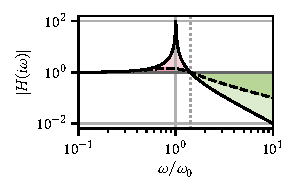
\includegraphics{img/pdf/setup/spring_tf}
    \caption[\imgsource{img/pdf/setup/springs.py}]{
        Force transmission function of a damped harmonic oscillator with $\gamma=\omega_0/100$ (solid black line) and $\gamma=\omega_0/2$ (dashed black line).
        Below the break frequency $\omega=\sqrt{2}\omega_0$ (dotted vertical line), external excitations are amplified (shaded red area).
        For larger damping $\gamma$, the amplification at resonance becomes smaller.
        Above $\omega=\sqrt{2}\omega_0$, excitations are attenuated (shaded green area).
        Both amplification below and attenuation above the break frequency become smaller as the damping rate $\gamma$ is increased.
    }
    \label{fig:setup:vibrations:spring:tf}
\end{marginfigure}

Let us adopt a simple toy model to gain an intuition for the behavior of a mass suspended on air springs as function of vibration frequency by modelling it as a damped harmonic oscillator.
Consider the displacement from equilibrium $x(t)$ of the test mass $m$ and switch on an external perturbation $u(t)$ acting on the \emph{base} of the spring, implying that the driving force experiences both the damping rate $\gamma$ and the spring stiffness $k=m\omega_0^2$ with $\omega_0$ the resonant frequency of the undamped system.
We can then compute the transfer function $H(s)$ from the Laplace transform of the Newtonian equation of motion,
\begin{equation}\label{eq:setup:spring:eom}
    \ddot{x}(t) + 2\gamma[\dot{x}(t)-\dot{u}(t)] + \omega_0^2 [x(t)-u(t)] = 0,
\end{equation}
yielding
\begin{equation}\label{eq:setup:spring:tf}
    H(s) = \frac{\hat{x}(s)}{\hat{u}(s)} = \frac{2\gamma s + \omega_0^2}{s^2 + 2\gamma s + \omega_0^2}.
\end{equation}
The magnitude of the transfer function evaluated at $s=\i\omega$ is shown in \cref{fig:setup:vibrations:spring:tf} for two different dampings, $\gamma = \omega_0/200$ (solid black line) and $\gamma = \omega_0/2$ (dashed black line).
Below $\omega=\sqrt{2}\omega_0$ (vertical dotted line), external impulses are in fact amplified.
The maximum at the damped system's resonance $\omega_{\mr{r}} = [\omega_0^2 - \gamma^2]^{\flatfrac{1}{2}}$ becomes smoothed out and smaller as the damping $\gamma$ is increased but never drops below unity.
This is the reason why resonance frequencies as small as possible are desirable in vibration isolation.
Above this frequency, the system initially attenuates with \qty{40}{\decibel} per decade up to $\omega=\omega_0^2/(2\gamma)$ and with \qty{20}{\decibel} per decade beyond for $\gamma/\omega_0\to 0$ (the underdamped case).
In the strongly damped case ($\gamma/\omega_0\to\infty$) the attenuation is only \qty{20}{\decibel} per decade starting at $\omega = 2\gamma$.

From \cref{eq:setup:spring:tf,fig:setup:vibrations:spring:tf}, we can infer two possible approaches to isolating a mass from vibrations.
The first is to make the system's resonance frequency $\omega_0$ as small as possible by resting it on a spring damping system.
This maximizes the region in which external influences are attenuated.
The second is to do the opposite, \ie, make the entire system as stiff (large $k$) and thereby $\omega_0$ as large as possible.
While this minimizes the attenuation region, it also moves the amplification region close to the resonance to higher frequencies, and possibly further away from the external excitation.
Consequently, this approach makes most sense if it is known that low-frequency excitations are the dominant source of vibrations.

A widely used metric for the isolation demand of vibration-sensitive equipment are the so-called \acrfullpl{vc}~\cite{Gordon1992,Gordon1999}.
These are design standard specifications for buildings housing, for example, lithography tools.
The \glspl{vc} are defined in terms of band-limited \gls{rms} values similar to what I have used in \thethesis (\cf \cref{eq:setup:vibrations:rms,eq:speck:psd:bandpower}).
However, instead of computing the band-limited \gls{rms} with a fixed lower band edge, one uses bands of a fixed width, typically over one-third of an octave.
To be specific, the one-third octave is defined in terms of its midband frequency $f_{\mr{m}}$ as the interval
\begin{equation}\label{eq:setup:vibrations:third_octave}
    f\in f_{\mr{m}}\times\left[10^{-\flatfrac{1}{20}},10^{\flatfrac{1}{20}}\right] \approx f_{\mr{m}}\times\left[2^{-\flatfrac{1}{6}},2^{\flatfrac{1}{6}}\right]
\end{equation}
whose bandwidth \df is approximately \qty{26}{\percent} larger than $f_{\mr{m}}$ and where the latter is defined referenced to \qty{1000}{\hertz}~\cite{ansi_octave_bands}.
The criteria, given as velocities rather than displacements or accelerations because it is argued that the limit to photolithography resolution is image velocity, are reproduced from \citer{Gordon1999} in \cref{tab:setup:vibrations:vc}.
For the typical feature sizes we would like our microscope to resolve, the \acrshort{vc}-B criterion is a fair target.
I will use them below to classify the vibration isolation of the confocal microscope.

\begin{margintable}[*-12]
    \centering
    \footnotesize
    \caption{\Glspl{vc} and \gls{iso} guidelines~\cite{Gordon1999}.}
    \label{tab:setup:vibrations:vc}
    \begin{tabular}{ c @{}S@{} }
        \toprule
        \multicolumn{2}{l}{$\flatfrac{1}{3}$ \textsc{octave band \gls{rms} (\unit{\micro\meter\per\second})}} \\
        \midrule
        Workshop (\acrshort{iso})        & 800  \\
        Office (\acrshort{iso})          & 400  \\
        Residential day (\acrshort{iso}) & 200  \\
        Op. theater (\acrshort{iso})     & 100  \\
        \acrshort{vc}-A                  & 50   \\
        \acrshort{vc}-B                  & 25   \\
        \acrshort{vc}-C                  & 12.5 \\
        \acrshort{vc}-D                  & 6    \\
        \acrshort{vc}-E                  & 3    \\
        \bottomrule
    \end{tabular}
\end{margintable}

\subsection{Microscope isolation concept}\label{subsec:setup:vibrations:isolation:concept}
What does this mean for our case of a dry \gls{dr}?
The rotary valve motor of the \gls{ptr} generates pulses with frequency \qty{1.4}{\hertz}.
Commercial damping systems that the space constraints in our lab allow to be accommodated, for example the CFM Schiller MAS 25~\cite{CFMSchiller}, have resonance frequencies around $f_0 = \qty{2.5}{\hertz}$, implying the first two harmonics of the \gls{ptr} excitation fall into the amplification regime as discussed above.
We are thus right in-between the two regimes and it is a-priori unclear which isolation scheme to choose without detailed mechanics simulations.
Hence, the initial isolation concept for the cryostat envisaged mounting the rotary valve motor rigidly to the stiff aluminium item profile frame, which was additionally filled with sand to increase the system's resonance frequency.

However, prompted by a sudden increase in visually observed vibrations in the microscope image, I modified the cryostat frame to house three air springs~\sidecite{CFMSchiller} in the hopes of isolating the microscope from external disturbances.\sidenote{
    As it turned out, the cause was a damaged nanopositioner bearing rather than environmental.
    Fortuitiously, the endeavour still proved successful and resulted in an improved vibration performance as I show below.
}
To this end, I decoupled the frame from which the cryostat itself is suspended from the support frame standing on the lab ground.
Extruding from the square footprint of the support frame at two adjacent corners and the center of the diametrically opposite side, the three air springs are mounted with the base on angle brackets connected to the support frame while their plunger is mounted to a second angle bracket connected to the cryostat frame.
The springs are connected by pneumatic tubing to a central pressure regulation panel that is connected to the building's central air pressure line.
The vertical placement of the springs is chosen such that when the air springs are deflated the cryostat frame rests on the support frame, establishing the same rigid connection that existed previously.
This allows examining the influence of the air springs on the vibration isolation without modifying the setup by simply venting the pressurized air from the springs.

In the following, I will characterize the performance of the system with and without the air springs active using two different methods.

\section{Accelerometric vibration spectroscopy}\label{sec:setup:vibrations:accel}
The most straightforward method of measuring vibration noise is an accelerometer.
These are devices that convert translational forces, for example by means of a loaded spring, into electrical signals.
They are mounted rigidly to the \gls{dut} and typically connected to some sort of signal conditioner providing a constant current bias to the sensor and putting out a voltage proportional to the acceleration.
The most sensitive and low-frequency designs use piezoelectric materials like Quartz crystals for sensitivities in the range of \qty{10}{\volt\per\gaccel} with a broadband noise floor of \qty{2}{\micro\gaccel}~\cite{WilcoxonAccel}.

In order to evaluate the vibration level at the sample position, I designed a small angle bracket onto which the accelerometer\sidenote{
    \accelerometer kindly lent by Marcus Eßer~\cite{WilcoxonAccel}.
}
can be screwed either in vertical or horizontal direction in the sample puck of the \gls{dr}, enabling measurements of the displacement noise along the direction of gravity as well as perpendicular to it and the optical axis.
The accelerometer is connected to the coaxial cables installed in the cryostat via an adapter cable from imperial 10-32 to \gls{sma} connector.
Outside of the cryostat, the signal is routed to a signal conditioner that provides the necessary current bias and outputs a voltage which is digitized by a \thedmm \gls{dmm} connected to the measurement computer.
Since the sensor's (conditioned) output is a voltage directly proportional to the acceleration, it is straightforward to compute the displacement \gls{psd} from time series data measured with the \gls{dmm} using the \pyspeck package presented in \cref{ch:speck:software}~\cite{Hangleiter_pyspeck}.
Leveraging the \code{fourier_procfn} argument, we can transform the voltage data first to acceleration and then, by integration, to displacement in frequency space as indicated in \cref{lst:setup:vibrations:accel}.

\begin{marginlisting}
    \begin{py}[
        fontsize=\footnotesize,
        breaklines,%
        breakafter=.,%
    ]
        from qutil.signal_processing import fourier_space
        from qutil.functools import chain, scaled
        from qutil import const

        sensitivity = scaled(1 / 9.9 / const.g)
        fourier_procfn = chain(
            sensitivity,
            fourier_space.derivative
        )
    \end{py}
    \caption{Functionality to transform the conditioned voltage to displacement in Fourier space.}
    \label{lst:setup:vibrations:accel}
\end{marginlisting}
\begin{figure}
    \centering
    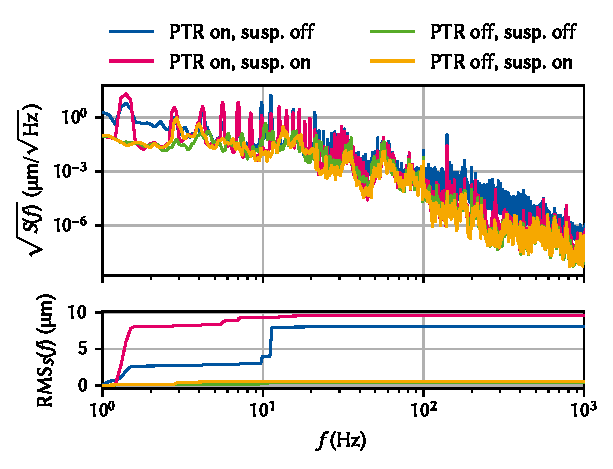
\includegraphics{img/pdf/setup/spect_accel}
    \caption[\imgsource{img/py/setup/vibration_spectroscopy.py}]{
        Top: displacement noise spectra acquired with the accelerometer at room temperature when the \gls{ptr} is switched on (blue, magenta) or off (green and orange), and when the air suspension is switched enabled (magenta, orange) or disabled (blue, green).
        Bottom: band-limited \gls{rms} computed from the \glspl{psd} in the upper panel (\cf \cref{eq:speck:psd:bandpower}).
        Turning on the \gls{ptr} increases the \gls{rms} noise amplitude by more than an order of magnitude over the entire frequency spectrum.
        The suspension slightly worsens the total noise because the low-frequency pulses excite the system close to the air springs' resonance frequency of \qty{2.5}{\hertz}.
    }
    \label{fig:setup:vibrations:accel}
\end{figure}

To assess the impact of the \gls{ptr} and the suspension, I measured the displacement noise \gls{psd} for each combination of the two being switched on and off.
The cryostat was closed, its vacuum chamber evacuated, and the magnet, a significant seismic mass, mounted as usual.
The measurements are shown in \cref{fig:setup:vibrations:accel} together with the band-limited \gls{rms} (\cf \cref{eq:speck:psd:bandpower}),
\begin{equation}\label{eq:setup:vibrations:rms}
    \rms_S(f) = \sqrt{\int_{f_\mr{min}}^{f}\dd{f^\prime}S^2(f^\prime)}.
\end{equation}
When the \gls{ptr} is switched off, the spectra with and without suspension are dominated by broadband vibration noise, although quite some structure around \qtylist{15;33;60}{\hertz} can be observed.\sidenote{
    Note the curious peaks slightly offset from the second and third harmonic of the \gls{ptr} frequency in the spectrum with suspension enabled and \gls{ptr} disabled.
    We may speculate that these are due to the \glspl{ptr} of other cryostats in other labs in the vicinity that are transmitted through the floor.
    Two were running two rooms over at the time the data was acquired.
}
When it is switched on, the \gls{ptr} pulses at \qty{1.4}{\hertz} and a large number of its higher harmonics visually dominate the spectra.
Clearly, the suspension has a larger impact in this case, matching qualitatively the behavior discussed in \cref{sec:setup:vibrations:isolation}.
At high frequencies, it manages to almost completely suppress the broadband excitation observed without the suspension.
At low frequencies, on the other hand, the \gls{ptr} harmonics are amplified to the degree that the band-limited \gls{rms} is dominated by their contribution.
Only at around \qty{10}{\hertz}, the attenuation starts to take effect.
Overall, the \gls{ptr} is found to raise the displacement noise \gls{rms} amplitude from \qty{0.5}{\micro\meter} to \qty{10}{\micro\meter} while the suspension, over the entire frequency range, has at best no positive influence.

This result is less than encouraging.
At that level of \gls{rms}-fluctuations, we'd have a slim chance of resolving micrometer-scale features using the microscope.
But is the \emph{absolute} magnitude of displacement noise at the sample position really the correct measure for the microscope performance?
Indeed, if the sample oscillates in phase with the objective and ocular lenses as well as the \gls{smf}, we will still obtain a perfect imaging fidelity.
So actually only the \emph{relative} displacements of sample, lenses, and detection fiber affect the achievable resolution of the microscope.
To characterize these, I developed an optical \emph{in-situ} technique to measure the displacement noise based on knife-edge reflectance fluctuations that I will present in the following section.

\section{Optical vibration spectroscopy}\label{sec:setup:vibrations:optic}
The gate electrodes on our samples are fabricated using two separate lithography processes; first, the smallest structures are written using \gls{ebl} in two steps.
Then, larger structures on the order of \qty{1}{\micro\meter} and above are written using optical lithography.
In the region where the two overlap on the mesa to establish electrical contact, the highly reflective \ch{Ti/Au} optical gates have a width of \qty{14}{\micro\meter} and a height of \qty{160}{\nano\meter} and lie on top of the poorly reflecting \ch{GaAs} surface, resulting in a step-like reflectance profile.
Scanning perpendicularly across such a straight edge between a poorly and a highly reflecting material is known as a knife-edge measurement and is frequently used to measure the spatial extent of a laser spot~\cite{Arnaud1971,Skinner1972,Khosrofian1983}.
We can use the same setup to measure the displacement noise; instead of manually shifting our knife edge across the beam spot, though, we measure the reflectance fluctuations induced by the knife edge fluctuating relative to the spot due to external perturbations.

\begin{marginfigure}[*-10]
    \centering
    \begin{tikzpicture}[
    round/.style={rounded corners=10pt},%
    font=\footnotesize,%
]

    % Mesa edge
    \draw[thick]
        (-2,0)
        -- ++(4.5,0)
    ;
    % Gate
    \path[draw=black, thick, fill=RWTHblack10, round]
        (-0.75,1)
        -- ++(0,-2.5)
        -- ++(1.5,0)
        -- ++(0,2.5)
    ;
    \path[draw=black, thick, dashed]
        (-0.75,1)
        -- ++(1.5,0)
    ;
    % Scan direction
    \draw[->, thick]
        (0.25,-0.75)
        -- ++(1,0) node[right] [align=center]{Scan \\ direction}
    ;
    % Laser spot
    \draw[dashed]
        (0.75,-0.75) circle (0.25)
    ;
    % Coordinate axes
    \draw[->]
        (1.75,0.3)
        -- ++(0.5,0) node[above] {$y$}
    ;
    \draw[->]
        (1.75,0.3)
        -- ++(0,0.5) node[right] {$z$}
    ;
    \draw
        (1.75,0.3) circle (0.1) node[left] {$x$}
    ;

    % Labels
    \node (mesa) at (-1.5,-0.25) {Mesa};
    \node (gate) at (0,0) [align=center]{Optical \\ gate};

\end{tikzpicture}
    \caption[\imgsource{img/tikz/setup/knife_edge.tex}]{
        Sketch of the region of the sample used for optical vibration spectroscopy.
        The coordinate system follows the magnet's; $z$ is parallel to gravity, and $x$ is perpendicular to the \gls{qw} plane.
        The optical gate extends further north as indicated by the dashed line.
    }
    \label{fig:setup:vibrations:knife_edge:sketch}
\end{marginfigure}

The scenario is sketched in \cref{fig:setup:vibrations:knife_edge:sketch} in the coordinate system defined by the magnet such that $z$ is along gravity's axis and $x$ is the out-of-plane axis.
Focusing the laser (indicated by a dashed circle) onto the edge of the optical gate, we can move the sample using the $y$-axis nanopositioner and observe a decrease in reflected intensity if the gate is moved away from the laser and an increase if it is moved towards the laser.
This gradient in reflected intensity can be inverted to obtain the vibration noise along $y$ by monitoring the intensity as a function of time.

Let us take a closer look at the reflected intensity when the laser spot has a finite overlap with the edge of the gate.
Under the simplifying assumption of a perfectly sharp drop-off and taking the reflectance of the Gold gate to be unity, we can write the reflectance as function of the coordinate perpendicular to the gate edge at $y=0$ as
\begin{equation}\label{eq:setup:reflectance_step}
    \reflectance(y) = \begin{dcases}
        1, & y \leq 0 \\
        \reflectance_0, & y > 0,
    \end{dcases}
\end{equation}
where $\reflectance_0$ is the reflectance of the bare \ch{GaAs} surface.
Assuming a perfect Gaussian (\gls{tem}$_{00}$ mode) beam characterized by its waist radius $w_0$ at which the intensity drops to $1/e^2$ of its maximum value, the laser intensity profile in 1D is given by
\begin{equation}\label{eq:setup:gaussian}
    I(y) = I_0\exp(-\frac{2y^2}{w_0^2}),
\end{equation}
where $I_0 = P_0/w_0$ with $P_0$ the total beam power.
The power reflected when the spot partially overlaps with the reflectance step can then be expressed as the convolution
\begin{equation}\label{eq:setup:knife_edge}
    P_{\mr{r}}(y) = \reflectance(y) \ast I(y) = \frac{I_0 w_0}{2}\sqrt{\frac{\pi}{2}}\left[ 1 - (1 - \reflectance_0)\erf\left(\frac{y\sqrt{2}}{w_0}\right) \right]
\end{equation}
in the $yz$ focal plane, where $\erf(y)$ is the error function.

\begin{marginfigure}
    \centering
    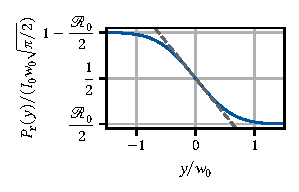
\includegraphics{img/pdf/setup/knife_edge_theory}
    \caption[\imgsource{img/py/setup/vibration_spectroscopy.py}]{
        Theoretical reflected power for a Gaussian beam of width $w_0$ and a reflectance contrast of $1-\reflectance_0$ according to \cref{eq:setup:knife_edge}.
        The dashed line indicates the leading order approximation at $y=0$.
    }
    \label{fig:setup:vibrations:knife_edge:theory}
\end{marginfigure}

The function is plotted in \Cref{fig:setup:vibrations:knife_edge:theory}.
The contrast that can be achieved is given by $1-\reflectance_0$.
Furthermore, for $y\in[-w_0/2, w_0/2]$ the function is well-approximated by
\begin{equation}\label{eq:setup:knife_edge:approx}
    P_{\mr{r}}(y)\approx -I_0(1-\reflectance_0)y + \frac{I_0 w_0}{2}\sqrt{\frac{\pi}{2}}
\end{equation}
drawn as a dashed line.
Since we measure the photon count rate rather than the power, $\Phi = \flatfrac{P\lambda}{hc}$ with $\lambda$ the laser wavelength, we rewrite this as
\begin{equation}\label{eq:setup:knife_edge:linearized}
    \Phi_{\mr{r}}(y) = -sy + \frac{\Phi_0}{2}\sqrt{\frac{\pi}{2}}.
\end{equation}
where we defined the \emph{sensitivity}
\begin{equation}\label{eq:setup:knife_edge:sensitivity}
    s = \frac{\Phi_0}{w_0}(1 - \reflectance_0).
\end{equation}
Hence, to obtain a more sensitive probe for vibrations, meaning that small variations in $y$ lead to large variations in $\Phi_{\mr{r}}$, one could either improve the reflectance contrast $1-\reflectance_0$, decrease the spot size $w_0$, or increase the incident photon flux $\Phi_0$.\sidenote{
    Note that the smaller $w_0$, the smaller also the maximum displacement amplitude that can be resolved as the derivative goes to zero as $y\to\pm\infty$.
}
In our case, the former two are fixed by the sample and the setup, respectively , whereas the latter is limited by the maximum data transfer rate of the \tagger counting card, \qty{9}{\mega\sample\per\second}.

Starting from \cref{eq:setup:knife_edge:linearized}, it is straightforward to obtain the displacement in the vicinity of $y=0$ as function of photon flux,
\begin{equation}\label{eq:setup:knife_edge:procfn}
     y(\Phi_{\mr{r}}) = \frac{w_0}{1-\reflectance_0}\left[\frac{1}{2}\sqrt{\frac{\pi}{2}} - \frac{\Phi_{\mr{r}}}{\Phi_0}\right].
\end{equation}
To summarize, we can position the laser spot on the edge of an optical gate and record a time trace of the photon flux by using the \taggershort to count the photons detected by the \glspl{apd} mounted on the side exit of the spectrometer.
Using \cref{eq:setup:knife_edge:procfn} we can then convert the flux into a displacement and proceed with the usual spectral noise estimation as explained in \cref{part:speck}.

\begin{marginfigure}[*-6]
    \centering
    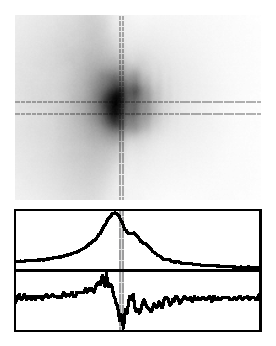
\includegraphics{img/pdf/setup/knife_edge}
    \caption[\imgsource{img/py/setup/vibration_spectroscopy.py}]{
        Calibration of the length reference scale.
        The top shows a \acrshort{cmos} camera image (higher intensity darker) of the white light spot on the edge of the optical gate as indicated in \cref{fig:setup:vibrations:knife_edge:sketch}.
        Several diffraction lines can be seen parallel to the edge.
        The vertical dashed lines indicate the region in which the intensity slope was fitted.
        The horizontal dashed lines indicate the extent of rows averaged over.
        The lower plots show a line cut along the central row of the considered region (top) and its derivative (bottom).
    }
    \label{fig:setup:vibrations:calibration:length_scale}
\end{marginfigure}

I will now lay out the experimental procedure of calibrating the system to (implicitly) obtain the parameters $w_0$, $\reflectance_0$, and $\Phi_0$.
The first challenge is obtaining a proper length reference scale.
While the nanopositioners on which the sample is mounted do in principle have a resistive position readout, it is extremely unreliable at small displacements.
Therefore, I calibrated the relative position using the imaging arm of the optical head.
\Cref{fig:setup:vibrations:calibration:length_scale} depicts the procedure.
Illuminating the sample with the white light, I positioned the spot on the edge of the optical gate and imaged the sample with the \cmoscam.
I then extracted the position of the edge, in pixels, for several rows to obtain some statistics by fitting a linear function to the edge profile in a small region between two refraction maxima.
Repeating this step for different DC voltages applied to the nanopositioner, this yields the proportionality factor between the nanopositioner DC voltage, $V_{\mr{DC}}$, and the position of the gate edge on the camera.
By measuring the total width of the gate on the camera image, I obtained the magnification by referencing it to the design width,
\begin{equation}\label{eq:setup:knife_edge:magnification}
    M = \frac{w[\unit{\pixel}]}{w[\unit{\micro\meter}]} = \frac{\qty{116}{\pixel}}{\qty{14}{\micro\meter}} \approx \qty{8.3}{\pixel\per\micro\meter}.
\end{equation}
Again performing a linear fit to the data for different voltages then results in the linear transformation from DC voltage to position (upper panel of \cref{fig:setup:vibrations:calibration:pos_vs_cps}).
Of course it is also possible to fit the full knife-edge function, \cref{eq:setup:knife_edge}, to the data shown in \cref{fig:setup:vibrations:calibration:pos_vs_cps}.
From this, the spot size $w_0$ and the actual bare \ch{GaAs} surface reflectance $\reflectance_0$ can be extracted.
Here we are content with the linear approximation; refer to \cref{subsec:app:setup:vibrations:knife_edge} for the full fits.

\begin{marginfigure}[*-7]
    \centering
    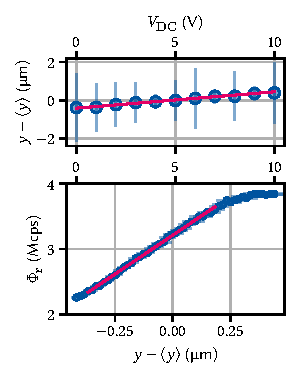
\includegraphics{img/pdf/setup/knife_edge_fits}
    \caption[\imgsource{img/py/setup/vibration_spectroscopy.py}]{
        Top: linear fit of the edge positions extracted from the analysis in \cref{fig:setup:vibrations:calibration:length_scale}.
        Error bars are propagated standard errors of the weighted average of edge positions extracted from different rows.
        Bottom: laser photon count rate as function of position set by the nanopositioner.
        Fitting the region $V_{\mr{DC}}\in[0.5, 7]\,\unit{\volt}$ yields $s\approx\qty{2.36+-0.02}{\mega\cps\per\micro\meter}$ (\cf \cref{eq:setup:knife_edge:linearized}).
        Error bars on $\Phi_{\mr{r}}$ show the standard error of the mean over multiple observations and error bars on $y$ show the fit error from the top panel.
    }
    \label{fig:setup:vibrations:calibration:pos_vs_cps}
\end{marginfigure}

Lastly, I switched from white light illumination to the laser, focused it onto the edge of a gate, and measured the photon count rate reflected off the sample as a function of $V_{\mr{DC}}$, from which we can finally extract the desired sensitivity (slope) $s\approx\qty{2.36+-0.02}{\mega\cps\per\micro\meter}$ of count rate over displacement.
The data and fit are shown in the bottom panel of \cref{fig:setup:vibrations:calibration:pos_vs_cps}.
Clearly, the count rate is linear in the displacement over a large range, indicating that for fluctuations with amplitude on the order of \qty{100}{\nano\meter} \gls{rms}, the measurement sensitivity should be sufficiently robust.

\begin{figure}
    \centering
    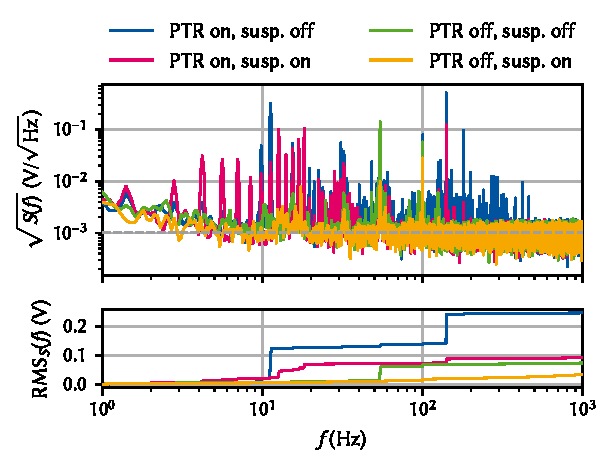
\includegraphics{img/pdf/setup/spect_optic}
    \caption[\imgsource{img/py/setup/vibration_spectroscopy.py}]{
        Top: displacement noise spectra acquired with the optical \emph{in-situ} method at room temperature when the \gls{ptr} is switched on (blue, magenta) or off (green and orange), and when the air suspension is switched enabled (magenta, orange) or disabled (blue, green).
        The dashed gray line indicates the theoretical noise floor derived in \cref{subsec:setup:vibrations:optic:noise_floor}.
        Bottom: band-limited \gls{rms} computed from the \glspl{psd} in the upper panel (\cf \cref{eq:speck:psd:bandpower}).
        The \gls{ptr} has a much smaller effect than when measuring the absolute displacement noise with the accelerometer, increasing the \gls{rms} only by a factor of two.
        While the lowest-order \gls{ptr} harmonics are amplified by up to an order of magnitude in amplitude with the suspension enabled, they contribute relatively little to the total \gls{rms} and are compensated by the superior high-frequency attenuation behavior.
        The total $\rms_S \approx \qty{100}{\nano\meter}$ with the cryostat in operation is below the typical \unit{\micro\meter} feature size.
    }
    \label{fig:setup:vibrations:optic}
\end{figure}

We are now at last able to measure the displacement noise using \pyspeck.
Setting \code{procfn} to the linear transformation given in \cref{eq:setup:knife_edge:procfn} and measuring the counts registered by the \glspl{apd} using the \taggershort,\sidenote[][*7]{
    Since the \glspl{apd} are arranged in a \gls{hbt} geometry, I combined the counts of both instruments using the virtual channel functionality of the \taggershort.
}
I obtained the displacement noise \glspl{psd} shown in \cref{fig:setup:vibrations:optic}.
A few things stand out.
First, rather than the $f^{-2}$ background observed with the accelerometer in \cref{sec:setup:vibrations:accel}, the noise floor is white ($S(f)=\text{const.}$) at approximately $\qty{1}{\nano\meter\per\sqrt{\hertz}}$.
To understand why, we need to take a closer look at the counting statistics, which we will postpone for a bit in order to first finish our discussion of the noise spectra.
Second, the overall noise level is much -- by a factor of 20 \gls{rms} -- lower than with the accelerometer.
We can attribute this to the fact that the optical method is sensitive to relative rather than absolute displacements.
If the cryostat and the optical head were infinitely stiff we would measure no displacement noise with this method -- intrinsic noise floor notwithstanding -- whereas the accelerometer is still sensitive to oscillations of the cryostat on the air spring fulcrum.
In that sense the optical method gives us the more pertinent results because only the displacements seen by the light travelling through the microscope ultimately matter.
Third, in contrast to the accelerometer measurements, the \gls{rms} amplitude is reduced by half when the suspension is active.
Although the harmonics of the \gls{ptr} frequency of \qty{1.4}{\hertz} are again amplified by the suspension below \qty{10}{\hertz}, raising the band-limited \gls{rms} above that with the suspension disabled, there occurs a crossover at the eighth harmonic frequency beyond which the attenuation outweighs the amplification at low frequency.\sidenote{
    It furthermore appears that even a measurement whose sole electronic device is a picosecond-resolution counting card cannot escape \qty{50}{\hertz} power line noise (or in this case its second harmonic).
}

\subsection{Noise floor}\label{subsec:setup:vibrations:optic:noise_floor}
The noise floor in the optical vibration measurements shown in \cref{fig:setup:vibrations:optic} is qualitatively very different from that observed with the accelerometer.
There, the \emph{acceleration} noise floor was white,\sidenote{
    Remember that as acceleration is the second time derviative of displacement, in frequency space it is proportional to $f^2$ times the latter.
}
whereas with the optical method the \emph{displacement} noise floor is white, hinting at a different underlying mechanism.

To elucidate this issue, we model the detection event of a single photon (a \enquote{click}) arriving at the detector at a random time $t_i$ as a $\delta$-function so that the total flux as function of time is given by
\begin{equation}\label{eq:setup:flux_comb}
    \Phi(t) = \sum_i \delta(t-t_i).
\end{equation}
Assuming them to be uncorrelated, the time difference between subsequent clicks is exponentially distributed with average rate $\bar{\Phi}$, $\lvert t_{i+1}-t_i\rvert\sim\expdist(\bar{\Phi})$~\cite{ExponentialDistributionWiki}.
From this it follows that the number of clicks $N(\dt)$ within a given time bin $t\in [s, u]$ of length $\dt = \lvert u - s\rvert$ is Poisson distributed, $N(\dt)\sim\poisson(\bar{N})$, with mean number of counts $\expval{N(\dt)} = \bar{N} = \bar{\Phi}\dt$~\cite{PoissonDistributionWiki}.
Using the formalism developed in \cref{sec:speck:theory:time_series_estimation}, we can now compute the \gls{psd} of the stochastic process $\delta N(\dt) = N(\dt) - \bar{N}$.
To this end, observe that because we assumed arrivals to be uncorrelated, $N_{u^\prime}(\dt)$ for a time bin starting at $t=u^\prime$ is independent of $N_{s^\prime}(\dt)$ for a time bin starting at $t=s^\prime$.
In other words, the autocorrelation function of $\delta N(\dt)$ is nonzero only for the same time bins,
\begin{equation}\label{eq:setup:poisson:autocorrelation}
    C_{\delta N(\dt)}(\tau) = \expval{(N_s(\dt) - \bar{N})(N_u(\dt) - \bar{N})} = \variance(N(\dt))\delta(\tau),
\end{equation}
where $\tau = s^\prime - u^\prime$ and $\delta(\tau)$ is to be understood in a broad sense as zero if $\abs{\tau} > \dt$ and $\flatfrac{1}{2\dt}$ else.
For the Poisson distribution the variance is equal to its mean so that we obtain
\begin{equation}\label{eq:setup:poisson:autocorrelation:evaluated}
    C_{\delta N(\dt)}(\tau) = \bar{N}\delta(\tau).
\end{equation}
In the limit of $\dt\to 0$, we can then perform the Fourier transform to obtain the \gls{psd} of $\delta N = \lim_{\dt\to 0}\delta N(\dt)$,\sidenote{
    Despite appearances, $S_{\delta N}$ has units \unit{\cts\squared\per\hertz}.
    The discrepancy stems from the difficulty in defining a continuous white noise process.
}
\begin{equation}\label{eq:setup:poisson:psd}
    S_{\delta N}(\omega) = \bar{N},
\end{equation}
that is, $\delta N$ is a white noise without frequency dependence.\sidenote{
    Note that we could have also arrived at this result directly by computing the autocorrelation function $\expval{\delta N(t)\delta N(t-\tau)}$ from \cref{eq:setup:flux_comb} with $N(t) = \int\dd{t}\Phi(t)$.
}
$S_{\delta N}$ can be seen as the \emph{instantaneous} number noise \gls{psd}.

As a last step, we consider once again discretely sampling the \emph{continuous} process $\delta N$ with \gls{psd} $S_{\delta N}(\omega)$ at rate $\fs=\dt\inverse$ in order to find an expression for the \gls{psd} of the discrete process $\delta N(\dt)$, $S_{\delta N(\dt)}(\omega)$.
We know from above that $\variance(\delta N(\dt)) = \bar{N}$.
On the other hand, recall from \cref{sec:speck:theory:time_series_estimation} that also
\begin{align}\label{eq:setup:shot_noise:var}
    \variance(\delta N(\dt)) = \intinf\ddf{\omega} S_{\delta N(\dt)}(\omega) = \int_{-\flatfrac{\fs}{2}}^{\flatfrac{\fs}{2}}\dd{f} S_{\delta N(\dt)}(f)
\end{align}
where the last equality holds true because of the finite bandwidth of the discretely sampled signal.
Since $S_{\delta N}$ is white, it follows that $S_{\delta N(\dt)}$ is, too, and we can directly evaluate \cref{eq:setup:shot_noise:var}, obtaining\sidenote{
    $S_{\delta N(\dt)}$ also has units \unit{\cts\squared\per\hertz}.
}
\begin{equation}\label{eq:setup:shot_noise:psd}
    S_{\delta N(\dt)}(\omega) = \frac{\bar{N}}{\fs}.
\end{equation}
To convert to the displacement noise \gls{psd}, we can simply convert units using the calibration derived above because if $N\sim\poisson(\bar{N})$ then so $y\sim\poisson(\flatfrac{\bar{N}\fs}{s})$ where $s$ is the slope of the calibration converting displacements to count rates, \ie, the sensitivity (see \cref{fig:setup:vibrations:calibration:pos_vs_cps,eq:setup:knife_edge:linearized}).
Hence,\sidenote{
    Note that this is the two-sided \gls{psd}; to convert to the one-sided version used in this chapter, multiply by two.
}
\begin{equation}\label{eq:setup:shot_noise:noise_floor}
   S_{\delta y(\dt)}(\omega) = \frac{\bar{N}}{\fs}\times\left(\frac{\fs}{s}\right)^2 = \frac{\bar{\Phi}}{s^2}
\end{equation}
with $\delta y = y - \expval{y}$.
This type of noise is known as \emph{shot noise}.
It was first studied in the context of electron transport by \citet{Schottky1918} and results from the discrete nature of, in our case, photons and their stochastic emission times~\cite{Blanter2000}.
For the parameters in the present measurements, $\bar{\Phi}\approx\qty{3}{\mega\cps}$ and $s\approx\qty{2.36}{\mega\cps\per\micro\meter}$ (\cf \cref{fig:setup:vibrations:calibration:pos_vs_cps}), we obtain a shot noise floor of $S_{\delta y(\dt)}\approx\qty{1}{\nano\meter\per\sqrt{\hertz}}$ in excellent agreement with the data shown in \cref{fig:setup:vibrations:optic} where the theoretical value is indicated by a gray dashed line.

Inserting the theoretical expectation for the sensitivity $s$, \cref{eq:setup:knife_edge:sensitivity}, into \cref{eq:setup:shot_noise:noise_floor}, we find that
\begin{equation}\label{eq:setup:shot_noise:noise_floor2}
    S_{\Delta y(\dt)}(\omega) = \frac{\epsilon}{\Phi_0}\left(\frac{w_0}{1-\reflectance_0}\right)^2
\end{equation}
if we identify $\bar{\Phi} = \epsilon\Phi_0$ for some (fixed) setup efficiency \eps.
This shows a clear path towards improving the \gls{snr} of the method.
Just as the sensitivity $s$ is improved by increasing $\bar{\Phi}$ and $1-\reflectance_0$ and by decreasing $w_0$, so is the shot noise floor, albeit quadratically in $w_0$ and $1-\reflectance_0$.
For example, for a reduction in spot size by a factor of two from inserting a different objective lens and a tenfold increase in maximum count rate achieved by replacing the counting card with a more powerful model,\sidenote{
    \swinst offers models with up to \qty{1.2}{\giga\sample\per\second}, although at that rate the jitter and dead time of the \glspl{apd} would start to become the limiting factors~\cite{SwabianTimeTagger}.
}
our simple model predicts a noise floor of $\qty{25}{\pico\meter\per\sqrt{\hertz}}$, a reduction by a factor of \num{40}.

To conclude this section, let us come back to the \acrlongpl{vc} defined in \cref{subsec:setup:vibrations:isolation:theory} and evaluate the microscope based on the two different measurement methods presented in this chapter.
The $\flatfrac{1}{3}$ octave band \gls{rms} velocities computed for the vibration spectra with \gls{ptr} enabled shown in \cref{fig:setup:vibrations:accel,fig:setup:vibrations:optic} are plotted in \cref{fig:setup:vibrations:vc}.
Based on the data from the accelerometer (circles), the microscope does not meet the targeted level of vibration isolation (\acrshort{vc}-B, solid gray line) over three octaves.
Because this method of measuring the vibration noise is sensitive to absolute changes, we can understand qualitatively why this is the case if we view the accelerometer at the sample position as the end of a large pendulum whose fulcrum is in the center of the plane spanned by the three air springs.
A rough estimate gives a resonant frequency of \qty{0.5}{\hertz},\sidenote{
    The center of mass sits close to the magnet approximately $l = \qty{1}{\meter}$ below the springs so that we have $f = (2\pi)\inverse\sqrt{\flatfrac{g}{l}}\approx\qty{0.5}{\hertz}$.
}
implying frequencies in the considered range, $[4, 32]\,\unit{\hertz}$, are fairly effective at exciting motion in the pendulum (\cf \cref{subsec:setup:vibrations:isolation:theory}).
By contrast, with the optical method we do not pick up on such motion because the ocular lens focusing the light into the \gls{smf} is fixed in the co-rotating frame with respect to our imagined pendulum.
Indeed, the \gls{vc} velocities computed for this method show that they are orders of magnitude smaller at low frequencies in particular since only deviations from the rigid body picture established above induce a change in signal.
Furthermore, the \gls{rms} is dominated by the broadband shot noise floor indicated by the loosely dashed dark gray line, implying that the true vibration-induced \gls{rms} is well below our targeted \acrshort{vc}-B criterion.

\begin{figure}
    \centering
    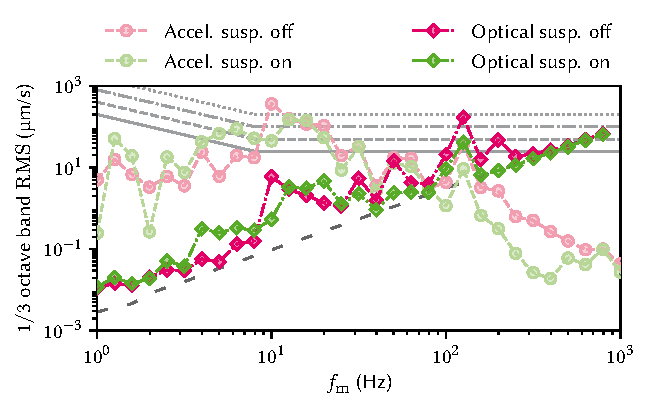
\includegraphics{img/pdf/setup/vc}
    \caption[\imgsource{img/pdf/setup/vibration_spectroscopy.py}]{
        $\flatfrac{1}{3}$ octave band \gls{rms} velocity computed for vibration measurements with the \gls{ptr} enabled and the suspension disabled (magenta) or enabled (green).
        Circles (diamonds) show data obtained with the accelerometer (optical method).
        The \glspl{vc} \acrshort{vc}-B, \acrshort{vc}-A and first two \gls{iso} levels are indicated as gray lines (solid, dashed, dash-dotted, dotted); see \cref{tab:setup:vibrations:vc}.
        Accelerometer data are above the \acrshort{vc}-B criterion for about three octaves centered around $f_{\mr{m}}=\qty{10}{\hertz}$, where even the \gls{iso} \enquote{residential day} level is breached.
        Optical data are more favorable, in particular with the suspension enabled (green).
        Towards high frequencies, the data are dominated by the wideband shot noise floor indicated by the loosely dashed dark gray line, suggesting the true displacement \gls{rms} is well below the \acrshort{vc}-B criterion.
    }
    \label{fig:setup:vibrations:vc}
\end{figure}

\section{Routes for improvement}\label{sec:setup:vibrations:outlook}
Several improvements could be made to the system if the external conditions would allow it.
First, the rotary valve motor should be moved further away from the cold head.\sidenote{
    Clearly, this will impact the performance of the \gls{ptr} to some extent and should therefore be considered carefully.
}
As per the initial installation status, it is currently connected to the cold head with a flexible hose at a right angle and a distance of roughly \qty{50}{\cm}, which is below the minimum bend radius recommended by \oxinst.\sidenote{
    Note that the orientation of the motor, which is horizontal with the axis, is also not the recommended configuration.
}
Additionally, the term \enquote{flexible} is relative here given the pressure of \qty{20}{\bar}.
Increasing the length of the hose should reduce its relative rigidity and thereby its ability to transmit vibrations from the motor to the cold head.

Next, the cold head should be mounted firmly to a secondary reference frame, for instance the ceiling or the lower cryostat frame on which the springs rest.
An intuitively obvious step, it has also been shown in the literature that decoupling the \gls{ptr} from the cryostat in this fashion leads to significant improvements in vibration isolation~\cite{Olivieri2017}.\sidenote{
    The former option was attempted, but showed no clear improvements in the measurements for reasons unclear, see \cref{sec:app:setup:vibrations} for additional data.
    It did emphatically deteriorate the inter-departmental atmosphere.
    Apologies to the institute on the floor above.
}
Acoustic insulation of the room and \gls{ptr} flex hoses could further improve the low-frequency response of the system~\cite{Schmoranzer2019,Oh2021}.
Lastly, let me note that there also exist cryocoolers with variable operating frequency that can thus be tuned away from problematic resonances in the system~\cite{TransMitPTR}.

In \cref{sec:app:setup:vibrations} I show additional spectroscopy data, including data measured along the gravitational axis in the puck and on the floor of different rooms, which suggests moving to a different laboratory could also benefit the vibration stability, as well as data for different configurations of the \gls{ptr} motor.
